% Copyright 2022  Ed Bueler

\documentclass[10pt,hyperref,dvipsnames]{beamer}

\mode<presentation>
{
  %\usetheme{Madrid}
  \usetheme{boxes}  % very plain and clean

  \usecolortheme{beaver}

  \setbeamercovered{transparent}
  
  \setbeamerfont{frametitle}{size=\large}
}

\setbeamercolor*{block title}{bg=red!10}
\setbeamercolor*{block body}{bg=red!5}

\usepackage[english]{babel}
\usepackage[latin1]{inputenc}
\usepackage{times}
\usepackage[T1]{fontenc}
% Or whatever. Note that the encoding and the font should match. If T1
% does not look nice, try deleting the line with the fontenc.

\usepackage{empheq}
\usepackage{animate}
\usepackage{xspace}
\usepackage{verbatim,fancyvrb}
\usepackage{tikz}
\usepackage{hyperref}

% If you wish to uncover everything in a step-wise fashion, uncomment
% the following command: 
%\beamerdefaultoverlayspecification{<+->}

\newcommand{\bb}{\mathbf{b}}
\newcommand{\bc}{\mathbf{c}}
\newcommand{\br}{\mathbf{r}}
\newcommand{\bx}{\mathbf{x}}
\newcommand{\by}{\mathbf{y}}
\newcommand{\bv}{\mathbf{v}}
\newcommand{\bu}{\mathbf{u}}
\newcommand{\bw}{\mathbf{w}}

\newcommand{\grad}{\nabla}

\newcommand{\CC}{\mathbb{C}}
\newcommand{\RR}{\mathbb{R}}

\newcommand{\ddt}[1]{\ensuremath{\frac{\partial #1}{\partial t}}}
\newcommand{\ddx}[1]{\ensuremath{\frac{\partial #1}{\partial x}}}
\renewcommand{\t}[1]{\texttt{#1}}
\newcommand{\Matlab}{\textsc{Matlab}\xspace}
\newcommand{\MO}{\Matlab}
\newcommand{\eps}{\epsilon}
\newcommand{\ds}{\displaystyle}


\newcommand{\mfile}[1]{
\VerbatimInput[frame=single,label=\fbox{\scriptsize \textsl{\,#1\,}},fontfamily=courier,fontsize=\scriptsize]{#1}
}

\newcommand{\mfiletiny}[1]{
\VerbatimInput[frame=single,label=\fbox{\scriptsize \textsl{\,#1\,}},fontfamily=courier,fontsize=\tiny]{#1}
}

\AtBeginSection[]
{
  \begin{frame}<beamer>
    \frametitle{Outline}
    \tableofcontents[currentsection,hideallsubsections]
  \end{frame}
}

\title{POPDIP}

\subtitle{a POsitive-variables Primal-Dual Interior Point \\ optimization method}

\author{Ed Bueler}

\institute[MATH 661]{MATH 661 Optimization}

\date{Fall 2022}

\begin{document}
\beamertemplatenavigationsymbolsempty

\begin{frame}
  \maketitle
\end{frame}


\begin{frame}{an example of a modern algorithm}

\begin{itemize}
\item POPDIP is a Newton-type primal-dual interior point algorithm
\item 1990s algorithm mostly covered in standard textbooks
    \begin{itemize}
    \item[$\circ$] section 16.7 in our textbook (Griva, Nash, \& Sofer, 2009)
    \item[$\circ$] chapter 19 in Nocedal \& Wright (2006)
    \end{itemize}
\item ``POPDIP'' is just my silly name for it \dots not an acronym in use

\bigskip
\item general problem it should solve:
\begin{equation*}
\begin{matrix}
\text{minimize} \qquad   & f(x) \\
\text{subject to} \qquad & A x = b \\
                         & x \ge 0
\end{matrix}
\end{equation*}

    \begin{itemize}
    \item[$\circ$] $f(x)$ must be smooth
    \item[$\circ$] user must provide $\grad f(x)$ and $\grad^2 f(x)$
    \item[$\circ$] $x\in \RR^n$, $A$ is a full row rank $m\times n$ matrix, $b\in\RR^m$
    \item[$\circ$] nonnegativity constraints $x\ge 0$ on \emph{all} variables
    \end{itemize}
\end{itemize}
\end{frame}


\begin{frame}{limitations}

\begin{itemize}
\item the POPDIP algorithm is suitable for:
\begin{equation*}
\begin{matrix}
\text{minimize} \qquad   & f(x) \\
\text{subject to} \qquad & A x = b \\
                         & x \ge 0
\end{matrix}
\end{equation*}
\item it is \emph{not} suitable for:
    \begin{itemize}
    \item[$\circ$] general equality constraints ``$g_i(x)=0$''
    \item[$\circ$] general inequality constraints ``$g_i(x)\ge 0$''
    \end{itemize}
\item see section 16.7 of Griva, Nash, \& Sofer (2009) for how to generalize it

\medskip
\item however, it \emph{can} be used as an interior-point method for linear programming (LP)
    \begin{itemize}
    \item[$\circ$] when $f(x)=c^\top x$ the problem is in LP standard form
    \item[$\circ$] but no special performance improvements for LP cases
    \end{itemize}
\end{itemize}
\end{frame}


\begin{frame}{decoding buzzwords}

\begin{center}
\emph{POPDIP is a {\color{BrickRed} Newton-type} {\color{OliveGreen} primal-dual} {\color{blue} interior point} algorithm}
\end{center}

\begin{itemize}
\item \emph{{\color{BrickRed} Newton-type}}: linearize $\grad f(x)$ and use the Hessian
    \begin{itemize}
    \item[$\circ$] compute $p$ so that $\grad f(x_k + p) \approx \grad f(x_k) + \grad^2 f(x_k) p = \dots$
    \end{itemize}
\item \emph{{\color{OliveGreen} primal-dual}}: keep track of $x$ \emph{and} Lagrange multipliers $\tau,\lambda$
    \begin{itemize}
    \item[$\circ$] Lagrangian is \qquad $\ds \mathcal{L}(x,\tau,\lambda) = f(x) - \tau^\top (Ax - b) - \lambda^\top x$
    \item[$\circ$] 1st-order KKT conditions:
\begin{align*}
\grad f(x) - A^\top \tau - \lambda &= 0 \\
-A x + b &= 0 \notag \\
\lambda_i x_i &=0, \qquad i=1,\dots,n \notag \\
x \ge 0, \quad \lambda &\ge 0 \notag
\end{align*}
    \end{itemize}
\item \emph{{\color{blue} interior point}}: iterates $x_k$ and $\lambda_k$ are in interior of feasible sets
    \begin{itemize}
    \item[$\circ$] this needs more explanation
    \end{itemize}

\medskip
\item more about the algorithm after example applications!
\end{itemize}
\end{frame}


\begin{frame}{example 1: $f$ quadratic, $n=2$, $m=0$}

\begin{itemize}
\item problem: \quad min $f(x) = \frac{1}{2} (x_1-1)^2 + \frac{1}{2} (x_2+1)^2$

\phantom{dsklfja dslfa} subject to $x \ge 0$

\bigskip
    \begin{itemize}
    \item[$\circ$] $\grad f(x) = (x_1-1,x_2+1)^\top$
    \item[$\circ$] unconstrained minimizer $(1,-1)^\top$
    \item[$\circ$] solution $x_*=(1,0)^\top$
    \end{itemize}

\vspace{-20mm}
\hfill
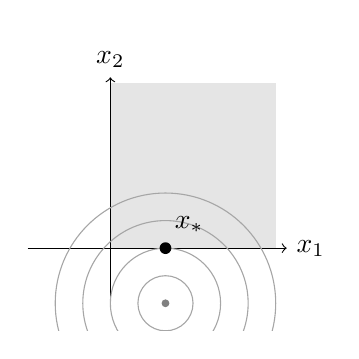
\begin{tikzpicture}[scale=0.7]
\clip (-1.5,-1.5) rectangle (4,4);
\fill[gray!20] (0,0) -- (3,0) -- (3,3) -- (0,3) -- cycle;
\draw [thin, ->] (-1.5,0)--(3.2,0) node[right] {$x_1$};
\draw [thin, ->] (0,-1.1)--(0,3.1) node[above]{$x_2$};
\foreach \r in {0.5,1.0,1.5,2.0}
    { \draw[gray!70] (1,-1) circle (\r); }
\node at (1,-1) [gray,circle,fill,inner sep=1.0pt]{};
\node at (1,0) [circle,fill,inner sep=1.5pt]{};
\node[xshift=3mm,yshift=+3mm] at (1,0) {$x_*$};
\end{tikzpicture}

\item Lagrangian and KKT conditions:
\begin{align*}
&& \grad f(x) - \lambda &= 0 \\
\mathcal{L}(x,\lambda) &= f(x) - \lambda^\top x & \lambda_i x_i &=0 \notag \\
&& x \ge 0, \quad \lambda &\ge 0 \notag
\end{align*}
\end{itemize}
\end{frame}


\begin{frame}[fragile]
\frametitle{example 1 (\texttt{small.m}) results}

\begin{itemize}
\item result starting from $x_0=(2,2)^\top$?
\item superlinear convergence:
\begin{Verbatim}[fontsize=\scriptsize]
>> small
        x_1                  x_2
  0:    2.000000000000000    2.000000000000000
  1:    1.641421356237309    0.641421356237310
  2:    1.245446520462486    0.245446520462486
  3:    1.069404818969903    0.069404818969903
  4:    1.013447008853577    0.013447008853577
  5:    1.000537794151783    0.000537794151783
  6:    1.000000867357066    0.000000867357066
  7:    1.000000000002257    0.000000000002257
  8:    1.000000000000000    0.000000000000000
\end{Verbatim}

\item note complementarity $x_i\lambda_i=0$ at solution

\medskip
\hfill
\mbox{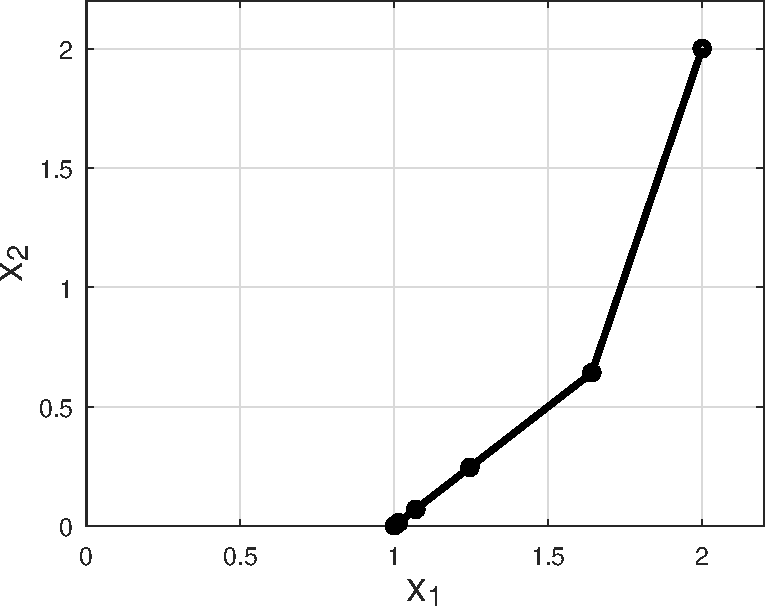
\includegraphics[width=0.4\textwidth]{figs/small.pdf} \qquad 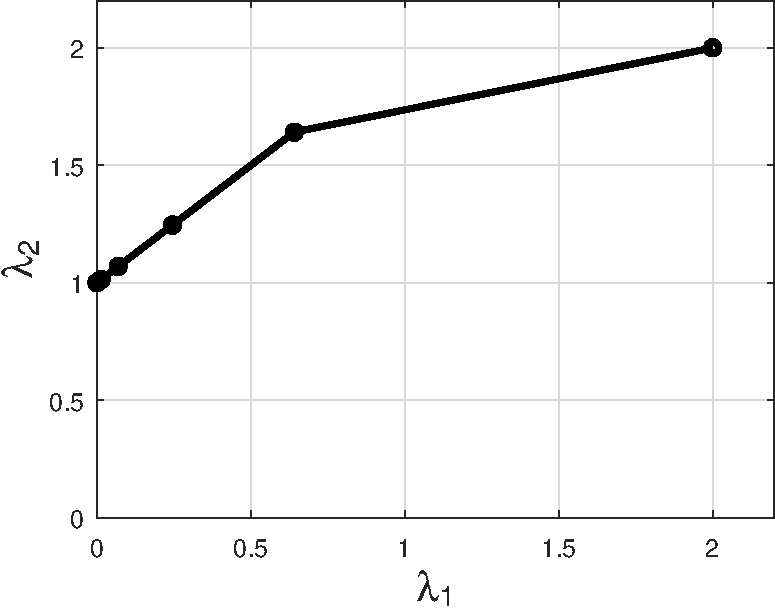
\includegraphics[width=0.4\textwidth]{figs/smalldual.pdf}}
\end{itemize}
\end{frame}


\begin{frame}{example 2: $f$ linear, $n=5$, $m=3$}

\begin{itemize}
\item remember our classic 2D LP problem?
\begin{equation*}
\begin{matrix}
\text{minimize} \qquad & z = -x_1 - 2x_2 \\
\text{subject to} \qquad & -2x_1 + x_2 \le 2 \\
 & -x_1 + 2x_2 \le 7 \\
 & x_1 \le 3 \\
 & x_1, x_2 \ge 0
\end{matrix}
\end{equation*}

    \begin{itemize}
    \item[$\circ$] section 5.2 uses this example to introduce simplex method
    \end{itemize}

\medskip
\item convert to standard form by adding slacks:
\begin{equation*}
\begin{matrix}
\text{minimize} \qquad & z = c^\top x \\
\text{subject to} \qquad & A x = b \\
 & x \ge 0
\end{matrix}
\end{equation*}

    \begin{itemize}
    \item[$\circ$] $\ds A = \begin{bmatrix} -2 & 1 & 1 & 0 & 0 \\ -1 & 2 & 0 & 1 & 0 \\ 1 & 0 & 0 & 0 & 1 \end{bmatrix}$, $\ds b = \begin{bmatrix} 2 \\ 7 \\ 3 \end{bmatrix}$, $c = \begin{bmatrix} -1 & -2 & 0 & 0 & 0 \end{bmatrix}^\top$
    \item[$\circ$] $\grad f(x) = c$, \quad $\grad^2 f(x)=0$
    \end{itemize}
\end{itemize}
\end{frame}


\begin{frame}[fragile]
\frametitle{example 2 (\texttt{linear.m}) results}

\begin{itemize}
\item results from starting at $x_0=(1,1)^\top$:
\begin{Verbatim}[fontsize=\scriptsize]
>> linear
        x_1                  x_2
  0:    1.000000000000000    1.000000000000000
  1:    1.749124060578910    3.650175187884218
  2:    2.771966360502739    4.813544496010846
  3:    2.977196636050274    4.937189711618397
  4:    2.993139910878286    4.988863175677374
  5:    2.999412769621014    4.999167116475287
  6:    2.999996717485349    4.999995406776724
  7:    2.999999999901378    4.999999999862158
  8:    3.000000000000000    5.000000000000000
\end{Verbatim}

\bigskip
\item internally, the POPDIP iteration is happening in 13-dimensional space!
    \begin{itemize}
    \item[$\circ$] $\mathcal{L}(x,\tau,\lambda) = c^\top x - \tau^\top (Ax - b) - \lambda^\top x$
    \item[$\circ$] $x_k \in \RR^5$, \quad $\tau_k \in \RR^3$, \quad $\lambda_k \in \RR^5$
    \end{itemize}
\end{itemize}
\end{frame}


\begin{frame}{example 2 (\texttt{linear.m}) results}

\begin{center}
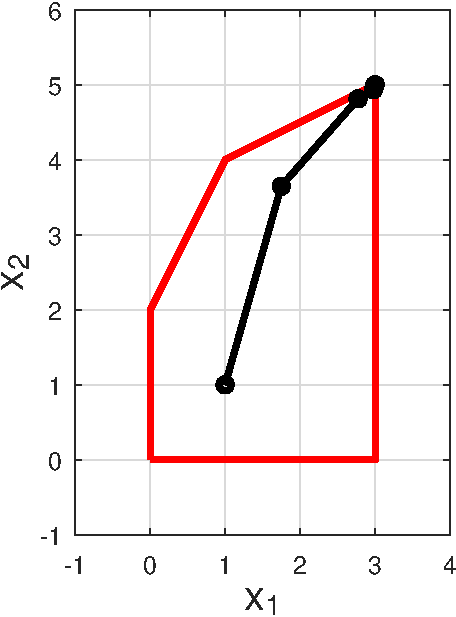
\includegraphics[width=0.4\textwidth]{figs/linear.pdf}
\end{center}
\end{frame}


\begin{frame}{example 3: $f$ quadratic, $n$ as large as you want, $m=0$}

\begin{itemize}
\item continuum problem is an \emph{obstacle problem}:
\begin{equation*}
\begin{matrix}
\text{minimize} \qquad & f(u) \\
\text{subject to} \qquad & u \ge 0
\end{matrix}
\end{equation*}
where \,\,$\ds f(u) = \int_0^1 \tfrac{1}{2} u'(x)^2 - q(x) u(x)\,dx$

    \begin{itemize}
    \item[$\circ$] consider only functions with zero end-point values:
    	$$S = \{v(x)\,:\, v(0)=v(1)=0 \text{ and } v(x) \ge 0\}$$
    \item[$\circ$] $n=+\infty$-dimensional problem
    \item[$\circ$] the obstacle is the zero function: $u\ge 0$
    \item[$\circ$] but $m=0$ \emph{equality} constraints
    \end{itemize}
\item discretize using piecewise-linear functions (finite elements):
\begin{equation*}
    f_n(u) = \Delta x \sum_{i=0}^n \tfrac{1}{2}\left(\frac{u_{i+1}-u_i}{\Delta x}\right)^2 - q(x_{i+\frac{1}{2}}) \frac{u_i + u_{i+1}}{2}
\end{equation*}

    \begin{itemize}
    \item[$\circ$] now $u\in\RR^n$ must have nonnegative entries ($u_i\ge 0$)
    \end{itemize}
\end{itemize}
\end{frame}


\begin{frame}{example 3: exactly-known continuum solution}

\begin{itemize}
\item testing is based on an exactly-known solution to the continuum problem
\end{itemize}

\medskip
\noindent
\hspace{-5mm}
\mbox{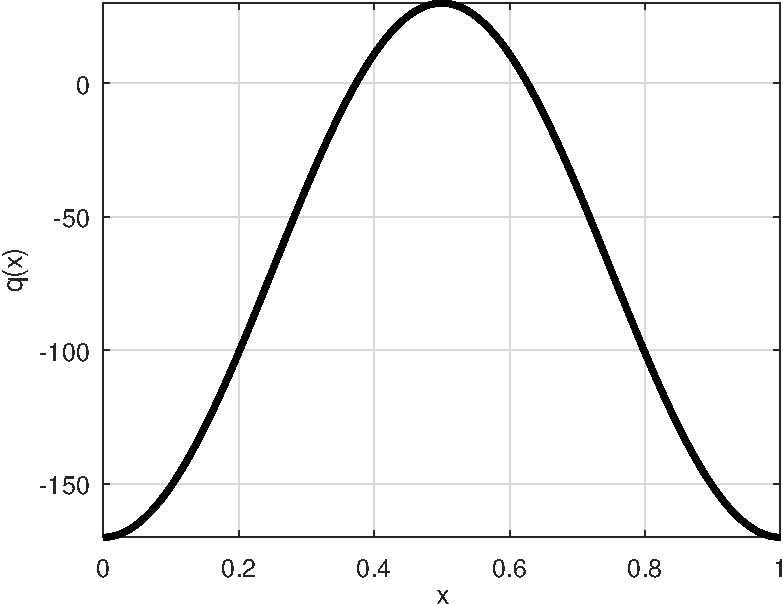
\includegraphics[width=0.5\textwidth]{figs/qobstacle.pdf} \qquad 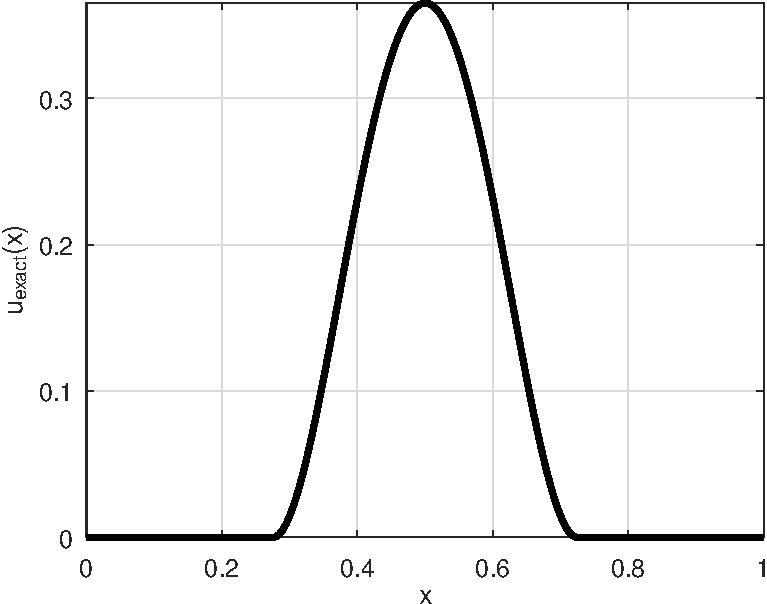
\includegraphics[width=0.5\textwidth]{figs/uexactobstacle.pdf}}
\end{frame}


\begin{frame}{example 3: results}

\begin{itemize}
\item results for $n=25$
\end{itemize}

\medskip
\begin{center}
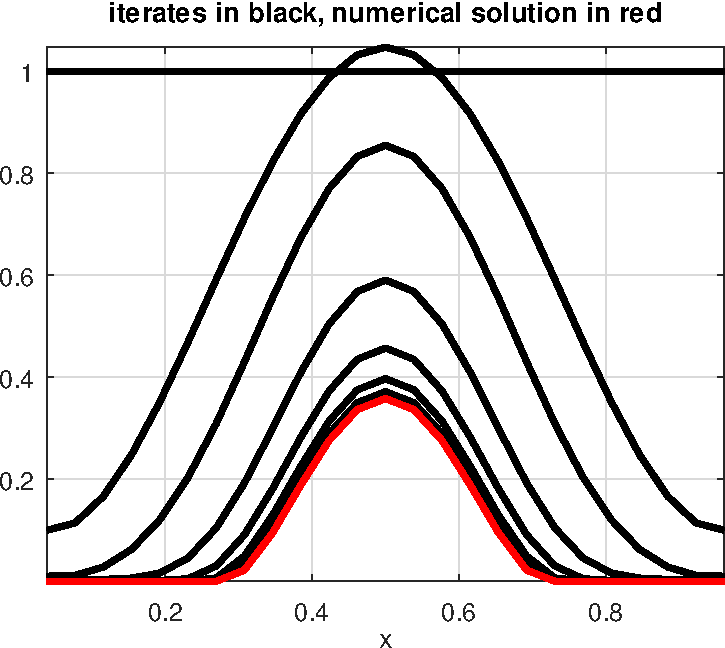
\includegraphics[width=0.7\textwidth]{figs/iteratesobstacle.pdf}
\end{center}
\end{frame}

\begin{frame}{example 3: results}

\begin{itemize}
\item results for $n=25$
\end{itemize}

\medskip
\begin{center}
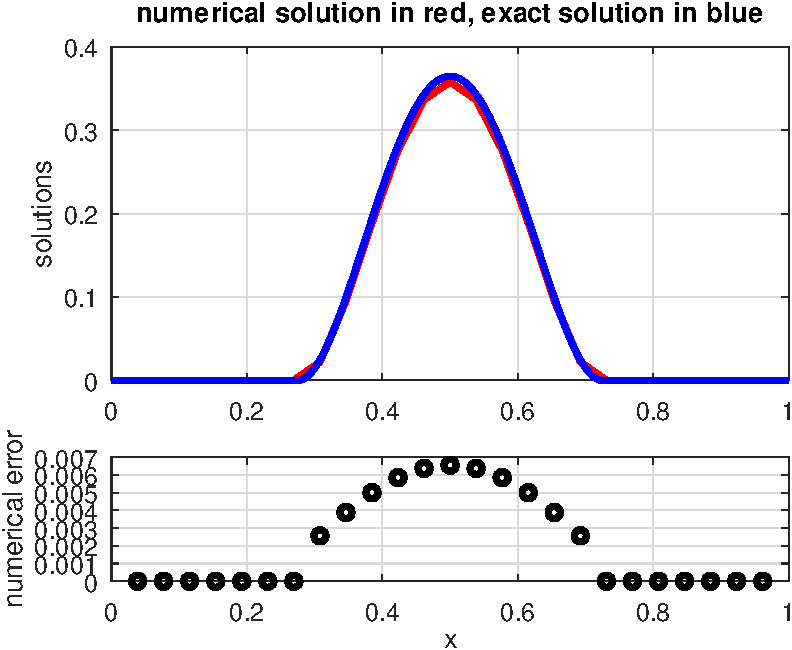
\includegraphics[width=0.8\textwidth]{figs/errorobstacle.pdf}
\end{center}
\end{frame}


\begin{frame}{how it works: modified KKT conditions explanation}

\begin{itemize}
\item y
\end{itemize}
\end{frame}


\begin{frame}{how it works: logarithmic barrier explanation}

\begin{itemize}
\item y
\end{itemize}
\end{frame}


\begin{frame}{fixme}

\begin{itemize}
\item the \alert{POPDIP algorithm}:

\medskip
\mbox{\parbox{\textwidth}{%
\begin{itemize}
\item[1.] User supplies $x_0$.

\medskip
\item[2.] For $k=0,1,2,\dots$
    \begin{itemize}
    \item[(i)] If $x_k$ is optimal then stop.

    \medskip
    \item[(ii)] Search direction is
       $$p_k = - \grad f(x_k)$$
    \item[(iii)] Determine step length $\alpha_k>0$.  Let $x_{k+1}=x_k+\alpha_k p_k$.
    \end{itemize}
\end{itemize}%
}}

\end{itemize}
\end{frame}


\begin{frame}{trying it yourself}

\begin{itemize}
\item clone the Github repository:

\begin{center}
\href{https://github.com/bueler/popdip}{\texttt{github.com/bueler/popdip}}
\end{center}

    \begin{itemize}
    \item[$\circ$] or download a \texttt{.zip} release from that website
    \end{itemize}

\item see the documentation PDF \texttt{doc.pdf} in the downloaded directory/folder
\end{itemize}
\end{frame}


\begin{frame}[fragile]
\frametitle{trying it yourself}

\begin{itemize}
\item POPDIP algorithm is a \Matlab function:

\medskip
\centerline{\texttt{function [x,tau,lam] = popdip(x0,f,A,b)}}

\medskip
    \begin{itemize}
    \item[$\circ$] input \texttt{x0} $\in\RR^n$ must have positive entries
    \item[$\circ$] inputs \texttt{A}, \texttt{b} are $m\times n$ and $m\times 1$
    \item[$\circ$] if \texttt{A=[]}, \texttt{b=[]} then $m=0$ and equality constraints are ignored
    \item[$\circ$] user-provided function \texttt{f} must have signature

\medskip
\centerline{\texttt{function [fx,dfx,Hfx] = f(x)}}

\medskip
    where \texttt{fx} $=f(x)$, \texttt{dfx} $=\grad f(x)$, \texttt{Hfx} $= \grad^2 f(x)$
    \item[$\circ$] output gives last iterate: \texttt{x} $\in\RR^n$, \texttt{tau} $\in\RR^m$, \texttt{lam} $\in\RR^n$
    \item[$\circ$] see \texttt{help popdip} for more control of solver parameters
    \end{itemize}

\item command line examples:
\begin{Verbatim}[fontsize=\small]
>> help popdip
>> small                          % run example 1
>> linear                         %     example 2
>> obstacle                       %     example 3
\end{Verbatim}
\end{itemize}
\end{frame}




\end{document}

